\section{Results}

To evaluate the performance of both models, several inferencing tests were conducted to see if the models had learned the latent features correctly.

\subsection{Recreation from the Training Dataset}

From each training dataset, a random frame was selected and passed through each model, loudness, F0 were kept constant. The results of the inferencing were then compared to the original training dataset.

Each model was able to successfully recrete original frames.

Timbral features were slightly distorted but the overall quality was good and it was easy to tell it was the original singer. Pitch estimation was highly accurate and in line with the original pitch. This can be partially attributed to the accruacy of the CREPE pitch detection model\cite{CREPE}.

A far bigger achievement was the re-synthesis of understandable words from the original frame. The original singing DDSP paper\cite{SingingDDSP} suffered a problem of stuttering when attempting resynthesis as their model was unable to recreate phonemes of the human voice accurately. It is possible that using far larger datasets has improved the quality of the resynthesis because the model has become more general in its ability to synthesize the human voice.

\begin{figure}
    \centering
    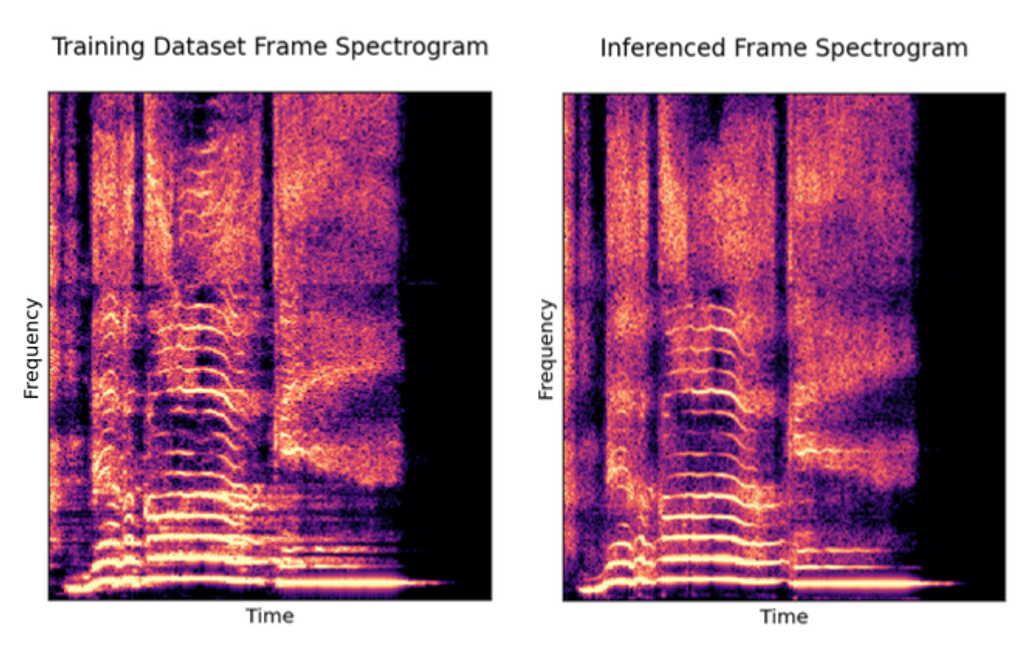
\includegraphics[width=0.8\textwidth]{research/results/TaylorSwift/InferredRecreation.png}
    \caption{(Taylor Swift) Original and resynthesized frames without latent modification}
\end{figure}

\subsection{F0 Pitch Transposition by a fixed octave}

A more advanced inferencing test was then undertaken, the fundamental frequency as determined by CREPE was transposed by fixed octaves (-2, -1, 0, 0.5, 1, 2) and the inferencing was re-preformed on the transposed frames.

At extreme transpositions, harmonics sometimes appeared to go silent. The resynthesis then appeared to sound like a whisper, coming almost entirely out of the filtered noise.

\begin{figure}
    \centering
    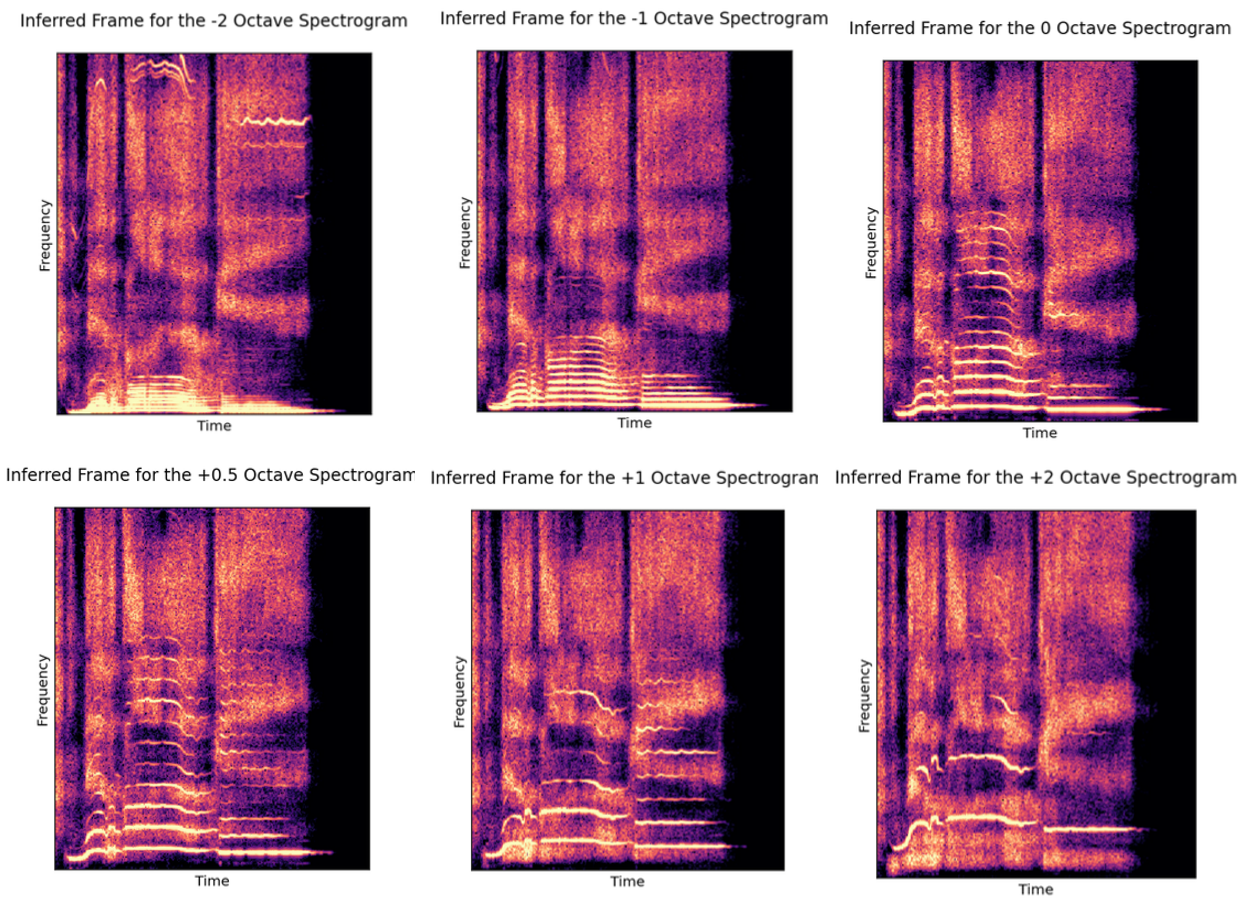
\includegraphics[width=\textwidth]{research/results/TaylorSwift/InferredTranspositions.png}
    \caption{(Taylor Swift) Inferred spectrogram frames at various octave transpositions realative to F0 at a certain timegrame in the original frame}
\end{figure}

\subsection{Fixing F0}

The final pitch related test was fixing F0 to the mean value of F0 throughout the frame to see how the models would perform under unnatural pitch conditions.

Both models were able to fix pitch to the mean value of F0 in the frame. This is clearly heard and can be seen visibily from the inferred spectrogram images where the harmonic components are at lines of constant frequency, unlike the orginial where they clearly vary.

This is a very good result mimicking what was founded in the Speech DDSP paper\cite{SpeechDDSP} (whose code wasn't publicly available). Further experimentations were done to vary the pitch to other amounts eg 100Hz 500Hz etc. to similar degrees of success, however the quality of results broke down at the extremes.

Additionally, words were still able to be synthesized and accurately heard, suggesting the model was able to learn the underlying phonemes of speech, or had at least learned how to pass them through the model.

Sadly, timbral quality was reduced when F0 was fixed, with the output sounding more robotic and the original timbre was lost. This is to be expected however as the original harmonic plus noise model was not designed with timbre transfer specifically in mind\cite{OriginalDDSP}.

\begin{figure}
    \centering
    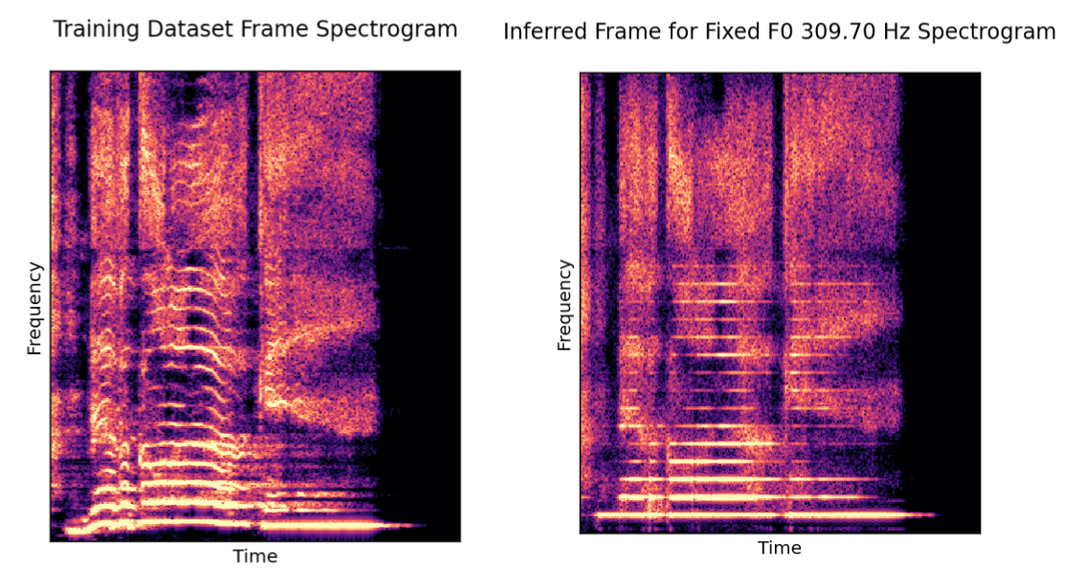
\includegraphics[width=\textwidth]{research/results/TaylorSwift/FixedF0.png}
    \caption{(Taylor Swift) Training dataset and fixed F0 spectrogram frames}
\end{figure}

\begin{figure}
    \centering
    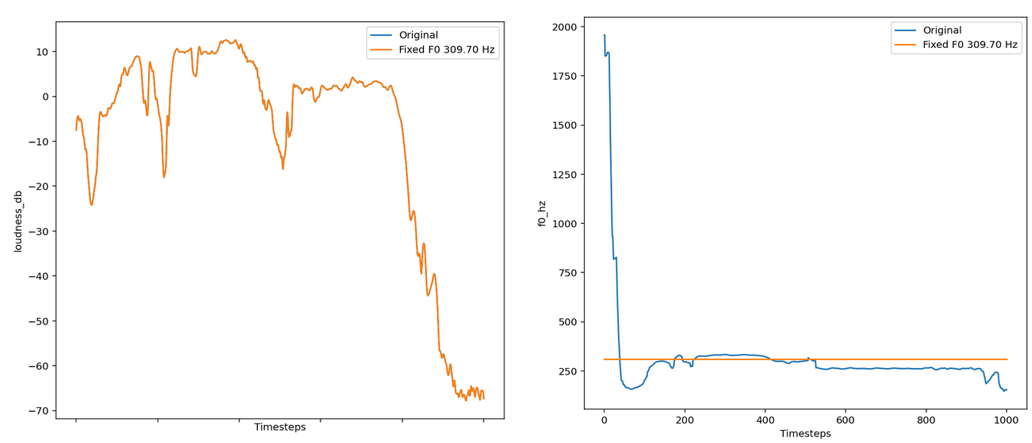
\includegraphics[width=\textwidth]{research/results/TaylorSwift/FixedF0Graphs.png}
    \caption{(Taylor Swift) Latent information on loudness and F0 over timesteps throughout the frame. The mean F0 was used to fix F0 throughout the frame}
\end{figure}